\section{Game Development} \label{sec:game-development}
As the complexity of games rose, game engines became more widely used \cite{blow2004game}. A game engine's goal is to reduce development time by enabling a collaborative process between programmers and artists, such that they can work together in one environment, to produce an application.
In \cite{Anderson:2008:CRG:1496984.1497031} the authors state that research, into engine development and architectures, is lacking. Another paper by the same author provides a good overview of what a game engine architecture, with a scripting system (see \figureref{typical-architecture}) may look like \cite{5962102}. Game engines commonly include the core subsystems seen in \figureref{engine-subsystes}.

\begin{figure}[H]
    \begin{subfigure}[b]{\textwidth}
        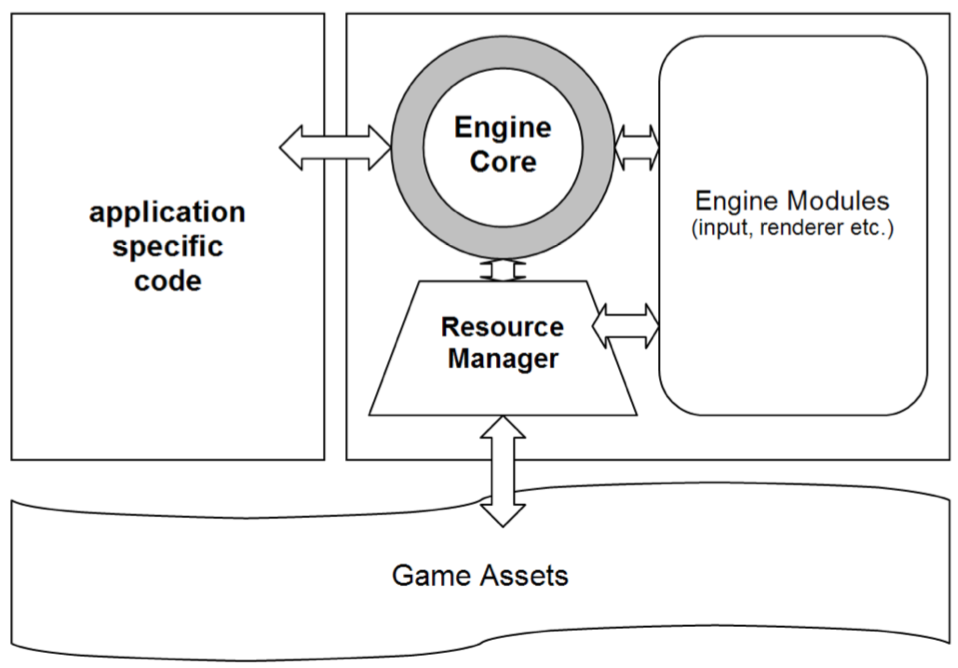
\includegraphics[width=\textwidth]{images/Game-development/Typical-game-engine.png}
        \caption{Typical game engine architecture with components \cite{5962102}.}
        \label{fig:typical-architecture}
    \end{subfigure}
    \begin{subfigure}[b]{\textwidth}
        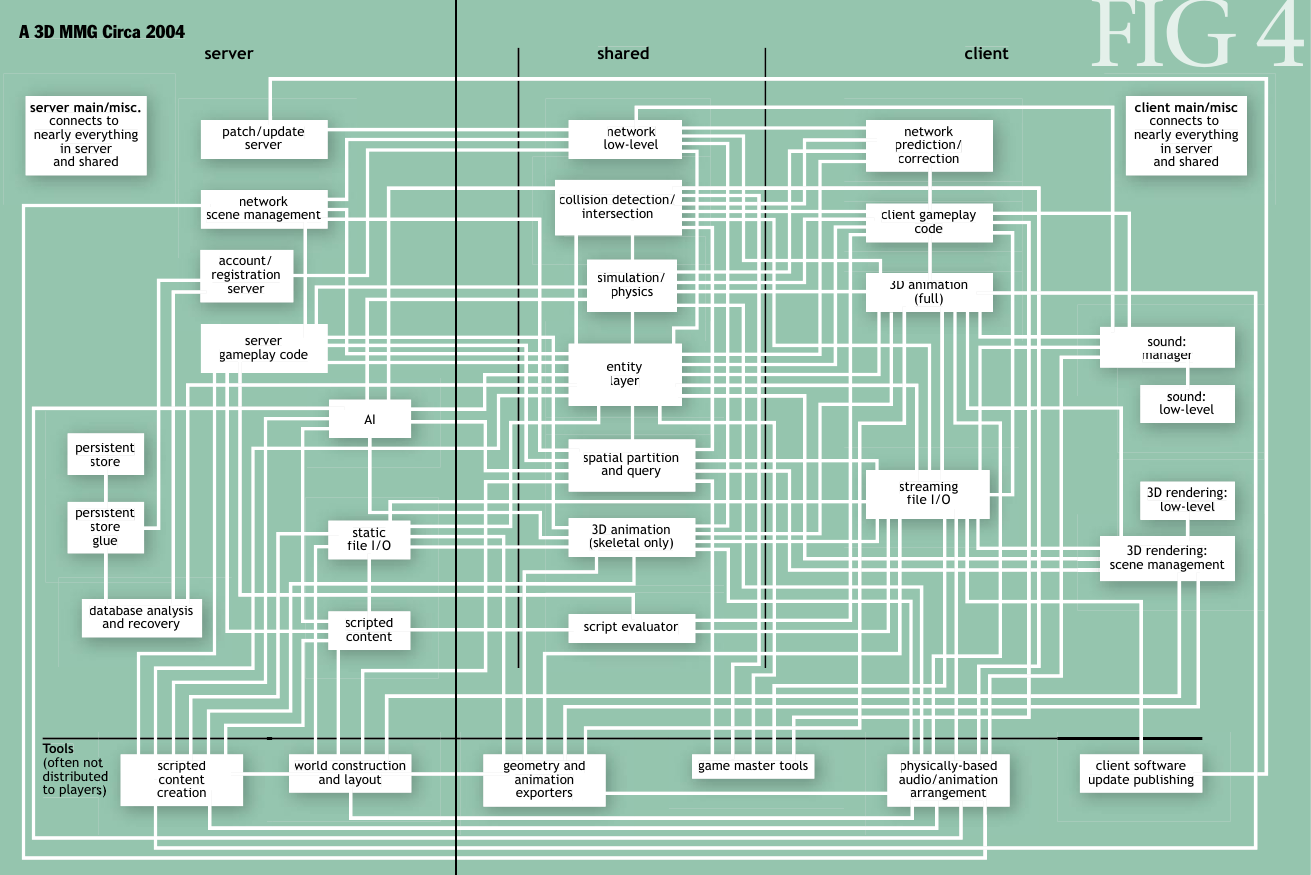
\includegraphics[width=\textwidth]{images/blow-complexity.png}
        \caption{Engine Code Complexity \cite{blow2004game}.}
        \label{fig:engine-compl}
    \end{subfigure}
    \caption{Game Engines, Theory and Practice.}
    \label{fig:engine-theo-prac}
\end{figure}

As game engines grew more complex, so did the subsystems of the engines \cite{blow2004game, nystrom2014game} (see \figureref{engine-compl}). Many of them are self-explanatory but the \textit{Core} system, of the engine, is a bit abstract. It is responsible for handling communication between the subsystems and ensuring correctness. It deals with memory management, file \ac{I/O} as well as handling startup of the game and all the associated devices \cite{nilson2007game}. 

\begin{figure}[H]
    \centering
    \begin{tasks}[style=itemize, column-sep=0mm, label-align=left, label-offset={0mm}, label-width={10mm}, item-indent={3mm}](3)%
        \task Audio
        \task Input
        \task Physics 
        \task Renderer
        \task Core
        \task Scripting
        \task Networking
        \task Artificial Intelligence
    \end{tasks}
    \caption{Engine Subsystems.}
    \label{fig:engine-subsystes}
\end{figure}

To showcase engine architecture, we will use the JOT engine as an example because it is an academic open source engine. JOT and its architecture is presented in \cite{amador2014jot}. JOT is a specialised modular multipurpose massively multiplayer online game engine \cite{amador2014jot}. The developers behind JOT had an interesting approach documenting their progress. The paper gave a design for JOT and specified the architecture, the whole project was for academic purposes.

JOT was implemented in Java, due to Java's multiplatform nature and the availability of third party applications and libraries. They also argue that there are already game engines, both for teaching and open source written in Java, so there would be a level of familiarity to the field. When looking at the JOT architecture (\figureref{Jot_layers}) it gives a clearer picture of each component needed, compared to that presented in \cite{5962102} (see \figureref{typical-architecture}). The figure defines what they make use of in their different components.

\subsubsection{Comparison}
Here we take a quick look at how JOT compares to the engine architecture from \cite{5962102} and the MMOG ecosystem put forward by \cite{blow2004game}.
We do this to see if game engines are constructed as described in the literature.

JOT provides many of the larger modules as displayed in \figureref{engine-compl}, although in larger modules. Note that the figure represents more than just the game engine, it's the whole system for a MMOG.
As it includes things such as persistent storage, separate client and servers, account registration, etc, it is not directly comparable with JOT.
It should however be possible to create both the game client and server with JOT, either by using the included modules or adding new ones.

There is some difference in the sub-division of modules between JOT and the engine architecture from \cite{5962102}. But in the coarse perspective they are similar. One way to attempt at fitting JOT into the model is the following (Engine architecture in bold, JOT in normal font): 
\begin{description} 
    \item[Engine Core] $\longleftrightarrow$ Infrastructure layer
    \item[Engine Modules] $\longleftrightarrow$ Modules from Core, (most of) Framework and Toolkit
    \item[Application specific code] $\longleftrightarrow$ Code that is above the framework layer in JOT
    \item[Resource Manager] $\longleftrightarrow$ (Part of) Managers from Framework layer
    \item[Game assets] $\longleftrightarrow$ Game assets
\end{description}

JOT is coarsely similar to the architecture and ecosystem presented by \cite{5962102} and \cite{blow2004game} respectively. There are minor differences in where components such as Physics and Rendering are placed, but overall they are similar.

\begin{figure}[H]
    \centering
    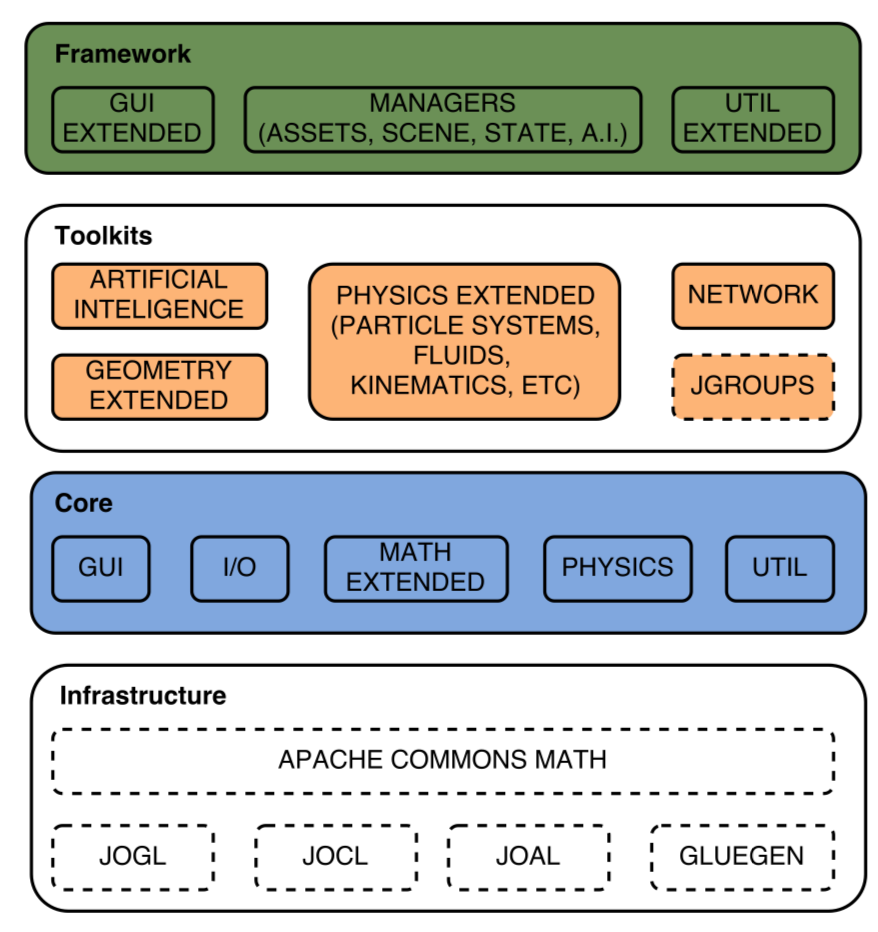
\includegraphics[scale = 0.6]{images/Game-development/Jot-layers.png}
    \caption{JOT architecture in layers \cite{amador2014jot}.}
    \label{fig:Jot_layers}
\end{figure}

When examining the core systems of a game engine, the programming language(s) is of particular interest in this project. The following section will examine scripting languages and what language(s) the game engine is implemented in.

\subsection{Gameplay Programming} \label{sec:gameplay:programming}
Gameplay programming often come in the form of scripting languages or \dquote{glue languages}. These are high-level languages used to develop game logic. They are one of the tools considered to be most important in modern game engines \cite{gamasutra:EngineSurvey, 5962102}. According to \cite{5962102} there is no clear definition of what a scripting language is, but they are generally used to control behaviour of other components. They often sacrifice run-time performance, in favour of writability. They often act as a layer of abstraction over subordinate components or programs \cite{5962102}.

Scripting systems make up a comprehensive list of applications and can be used in many different domains, depending on the application. Everything from command-line interpreters related to UNIX shells such as Ksh \cite{korn1994ksh}, to integrated scripting systems such as MEL(Maya Embedded Language) \cite{gould2003complete}, which for instance can be used to animate models in the Maya 3D graphics application.

Embedded scripting languages are often implemented for non-programmers \cite{gamedev:lua}. This is useful in game development, where a scripting system can be embedded in the computer game, which can be used to issue commands to the game engine such as loading objects, textures and levels, but also be used for more complicated tasks like playing an animated cut-scene or triggering events inside the game world. 
%A scripting language can also be embedded into the game engine, and give multiple uses.

According to \cite{5962102} the term scripting language is fuzzy and the authors propose a classification for scripting systems. This classification group script by what they are capable of solving. The categories are \cite{5962102}:
\begin{description}
    \item[Initialisation] are executed once during a program's run time, usually at the start. They are mostly used to set internal program parameters to the values given in the script.
    \item[Trigger-only] are split into event handler scripts and event oriented scripts. Both subcategories are used to execute scripts when a specific event happens in the game. \textbf{Event handler} scripts use events that are built into the game engine and define conditions on when to react to and what to do when a certain event occurs. \textbf{Event oriented} scripts are a bit more complicated. In these languages, the programmer defines triggers and conditions on when to react to certain events. Once every cycle the conditions are check and the appropriate triggers are invoked in case the conditions are met.
    \item[Program-like] defines two sub-categories; looping and regular scripts. Looping scripts are scripts that repeatedly execute, such that they keep reevaluating the current situation in the game. This means when the end of the script is reached, they restart execution from the beginning of the script. Regular scripts are scripts that execute once only. They will run from start to finish concurrently\footnote{It is not specified further in the source whether this is concurrency on multiple cores or thread-of-control} with the host application. But repeating operations, like loops, can be executed by the script.
\end{description}

\subsection{Engine Programming} \label{sec:engine:programming}
Industry game engines are often implemented in C++. The common belief with game developers is that C++ is a low-level, memory efficient language, used to get as much performance out of the hardware as possible\cite{gamasutra:c++functional}. According to Wikipedia C++ is used in many AAA studios and their engines, such as Unreal Engine 4 \cite{EpicGamesRepo}, Amazon Lumberyard \cite{awsRepo}, Unity3D \cite{wiki:Unity3D} and Frostbite \cite{wiki:Frostbite}.

Another language often used for open source and teaching material for game engine development is Java\cite{Java:Gamedev-tutorials}. It is of interest due to its multiplatform abilities, capabilities for multithreading and sockets\cite{amador2014jot}. Multithreading is important as \acp{CPU} no longer increase in clock frequency, but instead see an increase in the number of processing units, so it will lead to better utilisation of the \ac{CPU}\cite{Pfeffer2004}. Sockets provide a means for building multiplayer games \cite{freelancer:EngineLanguages}.

As an example, the original Minecraft game is implemented in Java. There also exist a C++ version, which was implemented by Microsoft after they bought the game \cite{pcgamersn:Minecraftinc++}. The general consensus in game development is that Java is not as favourable for game engine development as the garbage collector hinders performance, which is why it isn't used in big AAA game development \cite{gamasutra:MemoryHandling,youtubeJonathanBlow}.

%\subsection{Discussion}
%As we can see from our research\todo{not sure research is the right word} in game development as a field it is both very innovative\needcite, always using the newest technologies, adding new things on top of their game engine, to make games\todo[inline]{Bent skriver at dette ikke er tydeligt fra afsnittet. Jeg ved heller ikke personligt om jeg synes at vi har vist at noget er "innovativt"}. 
%But also very bound by tradition\footnote{Tradition here means the historical development process and tools of the industry.} and "what works". Why is it that game development is so obsessed with C++, and believe it is the most suited language for game engines.

%When they are so innovative and accepting of other technologies. Such as innovating new ways to make input to games, via new controllers, e.g. Wiimote or new modules such as \ac{VR} support to add complexity and new ways to give the user a fun gaming experience. At the foundation, game development uses C++ to make the underlying architecture, using arguments such as, they need as much performance as possible for their game engine\needcite.
%That they can't do what they do in C++, in other languages \cite{gamasutra:c++functional}.

%So they build these very effective game engines, pressing as much performance out of the hardware as possible, to then just put a scripting system on top, that is less effective and more sloppy with the use of memory\needcite.
%\todo[inline]{Bent skriver at det lyder populærvidenskabeligt, se forslag i kommentar.}

%Reasons why they are so stubborn using C++ may be that it is an industry that need to pump out as many games as possible to make a profit. So learning new technologies for their underlying systems might not be a priority when they can find good C++ programmers\todo{Excellent point, do we have a source?}.

%It might be that they think there is nothing better. Game development isn't a academic field, it is an industry. So reading the newest articles on development in language performance might not be relevant.
%So they are stuck thinking that C++ is the only language that can give them the performance they need\todo{This is conjecture}.